\begin{figure}[h]
\centering
\begin{minipage}{0.62\linewidth}
    \centering
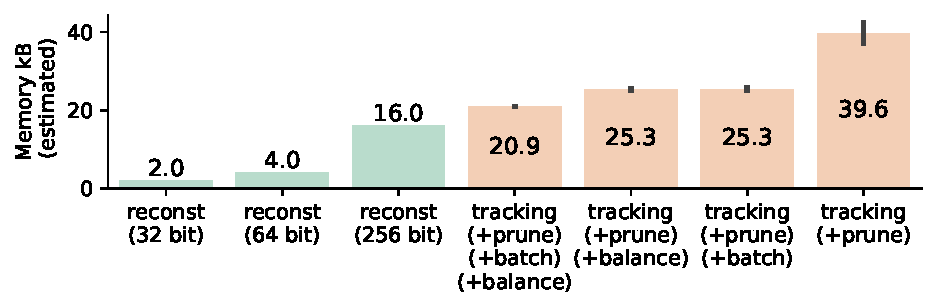
\includegraphics[width=0.95\linewidth]{binder/binder-2025-10-28-trafficsim_msprime.ipynb/binder/teeplots/2025-10-28-trafficsim_msprime/hue=flavor+viz=barplot+x=strategy+y=memory-use-kb+ext=.pdf}
\end{minipage}%
\begin{minipage}{0.38\linewidth}
\caption{%
\textbf{Per-node memory use for phylogeny tracking techniques.}
\footnotesize
Memory estimates for tracking approaches are estimated according to coalescent trees sampled using msprime, to simulate phylogeny migration dynamics across a processor grid.
We assume extinct lineages to be removed from memory through extinction tracking --- meaning that exact records need only be stored for extant lineages (pruning).
We assume unifurcations within the scope of a single PE are collapsed.
For batching optimization, it is assumed that the simulation is halted every 100,000 generations for a clean-up phase where data is offloaded off the chip to free on-chip memory from elapsed history.
For balancing optimization, it is assumed that memory load is shared evenly across the chip so that data capacity is necessary just on behalf of average behavior, not necessarily the most extreme cases requiring a buffer leeway.
Serial direct tracking represents a lower bound on memory usage for a bifurcating phylogeny, which scales as $2B$ population size.
A population size of 512 agents per node is assumed, with demes arranged in a 2D grid and agents migrating between neighboring demes at a rate of 5\%.
Further details on estimation methodology is provided in Section \ref{sec:TODO}.
}
\label{fig:msprime-memory-estimate}
\end{minipage}
\end{figure}
